\documentclass[11pt, a4paper]{article}
\usepackage{graphicx}  
\usepackage{url}
\usepackage{hyperref}
\usepackage{latexsym}
\usepackage{wrapfig}
\usepackage{float}
\usepackage{array}
\usepackage{enumitem}
\usepackage{amsmath} 
\usepackage{algorithm}
\usepackage{algpseudocode}
\usepackage{listings}

\hypersetup{
    colorlinks=true,
    linkcolor=blue,
    citecolor=green,
    filecolor=magenta,
    urlcolor=cyan,
}

\title{Informații preliminare - seminar}
\author{Cocu Matei-Iulian}
\date{20 sep. 2025}

\begin{document}
\maketitle

\section{Metodologie. Planuri de Învățământ}
\begin{itemize}
    \item \href{https://drive.google.com/drive/folders/1Rfsn9hPv4oCGH2hZljUB70Yoj0AQc_-U}{UB-FMI-Informatică}
    \item \href{https://drive.google.com/drive/folders/1YN07bNSGm6tsg8Xum497jAcJB5qQputp}{UB-FMI-CTI}
    \item \href{https://acs.pub.ro/public/CTI-C-Licenta.pdf}{UPB-ACS-CTI}
    \item \href{https://csie.ase.ro/programe/informatica-economica/}{ASE-CSIE-Informatică}
    \item \href{https://csie.ase.ro/programe/cibernetica-economica/}{ASE-CSIE-Cibernetică}
    \item \href{https://mateinfo.unitbv.ro/images/2024_/Planuri_Invatamant/Plan_inv_Matematica_informatica_2024_2027.pdf}{UNITBV-Informatică}
\end{itemize}

\section{Informații Admitere}
\begin{itemize}
    \item \href{https://fmi.unibuc.ro/admitere-licenta-iulie-2025/}{UB-FMI}
    \item \href{https://admitere.pub.ro/Admitere/site/alegeCentru}{UPB}
    \item \href{https://www.cs.ubbcluj.ro/admitere/nivel-licenta/admiterea-la-facultatea-de-matematica-si-informatica-nivel-licenta/}{UBB-FMI}
    \item \href{https://mateinfo.unitbv.ro/ro/admitere/admitere-licenta.html}{UNITBV}
\end{itemize}

\section{Subiecte (Pre)Admitere}
\begin{itemize}
    \item \href{http://www.physics.pub.ro/Admitere/subiecte.html}{UPB}
    \item \href{https://drive.google.com/file/d/1q_3gIfcSsQ0KRT0LRzlUHNC3dQFd9SC7/view}{Carte MateInfoUB}
    \item \href{https://www.cs.ubbcluj.ro/admitere/nivel-licenta/subiecte-din-anii-precedenti/}{UBB-FMI}
\end{itemize}

\newpage

\section{Probleme de rezolvat}
\subsection{Diverse}
\textbf{Problema 1}\newline
Ionel are 10 creioane. Lungimile fiecărui creion sunt: \[ 4, 3, 7, 8, 7, 4, 5, 8, 13, 15\]
El își dorește să obțină creioane având doar două lungimi diferite. Pentru a realiza acest lucru, el poate scurta (prin ascuțire) unele creioane.

\noindent Care este suma maximă a lungimilor creioanelor pe care o poate obține Ionel, după ce efectuează operațiile?
\vspace{1cm}

\textbf{Problema 2}\newline
Un număr \textbf{x} poate ajunge la un număr \textbf{y} (y \> x) trecând prin numerele dintre ele utilizând o secvență de pași. Lungimea fiecărui pas este pozitivă și poate fi egală cu lungimea pasului anterior, mai mare cu 1 sau mai mică cu 1. \textbf{Lungimile primului și ultimului oas trebuie să fie egale cu 1.}

\noindent Care este numărul minim de pași prin care se poate ajunge de la 2021 la 3110?
\vspace{1cm}

\textbf{Problema 3}\newline
Primarul P. are de acoperit un perete lung de 100 m și înalt de 1 m, pe care vrea să îl împânzească cu postere publicitare. În acest sens, a cumpărat 8 postere, de înălțime egală cu 1 m și lățimile (exprimate în metri):
\[ 12, 27, 13, 25, 26, 38, 28, 38 \]
El va trebui să aranjeze posterele de-a lungul peretelui. Posterele nu au voie să se suprapună și nu pot depăși marginile peretelui. Care este aria maximă de perete pe care o poate acoperi folosind posterele cumpărate?
\vspace{1cm}

\textbf{Problema 4}\newline
Un șir de caractere este \textit{plictisitor} dacă are lungime egală cu 7 și conține caractere din mulțimea {A, B}. Care este al 85-lea șir de caractere \textit{plictisitor} în ordine alfabetică?
\vspace{1cm}

\textbf{Problema 5}\newline
Care este suma maximă a elementelor matricei de mai jos, după înmulțirea unor linii și/sau coloane cu -1? Înmulțirea unei linii sau coloane cu -1 presupune înmulțirea tuturor elementelor sale cu -1.
\[
  \begin{pmatrix}
    4 & -1 & 6 & 4 & -5 \\
    -2 & -33 & -12 & 10 & -11 \\
    1 & 0 & 3 & -1 & 4 \\
    -99 & -98 & -40 & 34 & 33
  \end{pmatrix}
\]
\newpage

\textbf{Problema 6}\newline
Se dă matricea $A_{n \times n}$ (A este matrice cu $n$ linii și $n$ coloane) cu $n > 0$ și secvența de pseudocod următoare:
\begin{algorithmic}

\For{$i \gets 1$ \textbf{to} $n$}
    \For{$j \gets 1$ \textbf{to} $n$}
        \State $A_{ij} \gets (i+j) \pmod{n}$ 
    \EndFor
\EndFor

\end{algorithmic}
\noindent Care va fi suma elementelor de pe diagonala secundară a matricei \textit{A} în urma execuției secvenței?
% \vspace{1cm}

% \textbf{Problema 7}\newline

% \vspace{1cm}

% \textbf{Problema 8}\newline

% \vspace{1cm}

% \textbf{Problema 9}\newline

% \vspace{1cm}

% \textbf{Problema 10}\newline


\subsection{Complexitate}
\textbf{Problema 1}\newline
În pseudocodul următor \textit{n, s, i, j, k} sunt numere naturale:
\begin{algorithmic}
\State citește $n$
\State $s \gets 0$
\For{$i \gets 1$ \textbf{to} $n \cdot n$}
    \For{$j \gets 1$ \textbf{to} $i \text{ div } 2$}
        \State $A_{ij} \gets (i+j) \pmod{n}$
    \EndFor

    \State $k \gets 1$ 
    \While{$k < j$}
        \State $s \gets s + k$
        \State $k \gets k \cdot 2$
    \EndWhile
\EndFor

\State scrie $s$

\end{algorithmic}
\noindent Care este complexitatea secvenței de cod anterioare?
\vspace{1cm}

\textbf{Problema 2}\newline
în următoarea secvență de cod variabilele \textbf{i}, \textbf{j} și \textbf{k} sunt de tip întreg, iar \textbf{n} este un număr natural citit de la tastatură. Care este complexitatea timp a acestei secvențe de cod?
\begin{lstlisting}[language=C++]
k = 0;
for (i = n / 2; i <= n; i++)
    for (j = 2; j <= n; j = j * 2)
        k = k + n / 2;
\end{lstlisting}

\newpage
\subsection{Teoria Grafurilor}
\textbf{Problema 1}\newline
Pentru un graf G, un \textit{arbore parțial} este un graf conex, fără cicluri, conținând același număr de noduri ca G și doar muchii din G (dar nu neapărat toate).
Numărul de \textit{arbori parțiali} ai grafului de mai jos (reprezentand prin listă de adiacență) este egal cu:
\begin{enumerate}
    \item {3, 5}
    \item {4, 5}
    \item {1, 4, 5}
    \item {2, 3}
    \item {1, 2, 3}
\end{enumerate}

\textbf{Problema 2}\newline
Considerăm arborele din imagine:
\begin{figure*}[htbp]
    \centering
    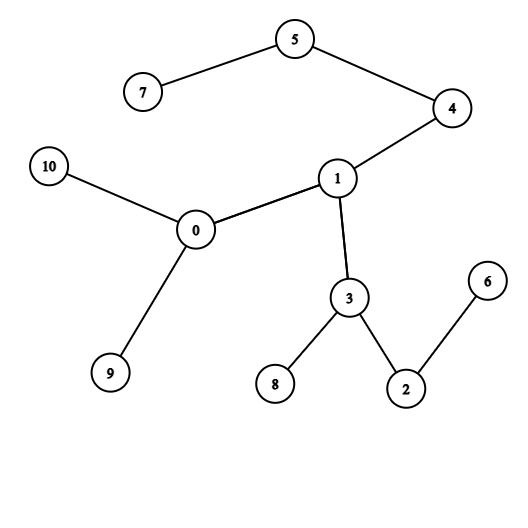
\includegraphics[width=0.39\textwidth]{graph.png}
\end{figure*}
Asupra sa putem aplica oricâte operații de două tipuri:
\begin{enumerate}
    \item ștergem o muchie;
    \item adăugăm o muchie.
\end{enumerate}
Care este numărul minim de operații care trebuie aplicate arborelui pentru a-l transforma într-un singur lanț care leagă cele 11 noduri?
% \vspace{1cm}

% \textbf{Problema 3}\newline

% \vspace{1cm}

% \textbf{Problema 4}\newline

% \vspace{1cm}

% \textbf{Problema 5}\newline


\end{document}